\section{\label{sec:beam:background} Beam background studies}
%\writer{Daniel Jeans, Yan Benhammou, Sergej Schuwalow, Claude Vallee}{2}
\label{ild:sec:beam_backgrounds}
The ILD detector response is affected by three main sources of beam-related background: beamstrahlung emitted at the crossing point of the electron and positron bunches, halo muons produced upstream of the detector along the beamline, and low energy neutrons back-scattered from the beam dumps. Their impact on the detector occupancies has been quantified and possible mitigation investigated\cite{ild:bib:Machine_Backgrounds,ild:bib:schuetz_thesis}. Results are similar for both options of the ILD detector and are shown here for the large version.

\subsection{Beamstrahlung}

Beamstrahlung photons are radiated from the ILC beam particles in the interaction with the electromagnetic fields of the strongly focused oncoming bunches. These photons can convert to $e^+e^-$ pairs with a broad energy spectrum. Most of the low-energy pairs are confined close to the z axis by the solenoid magnetic field but, due to the crossing angle between the colliding beams, a significant fraction hit the very forward detectors near the incoming and outgoing beam pipes. The central detectors are also affected, both directly by the $e^+e^-$ pairs, and indirectly through back-scattering of low-energy particles from the forward detectors. It was proposed to mitigate these effects by the addition of a small dipole field to the main solenoidal field. This so-called "anti-DID" field can be tuned to guide a large fraction of the  $e^+e^-$ pairs into the outgoing beampipe. 

These effects have been quantified for the updated 250 GeV ILC conditions (ILC250, see Section~\ref{ild:sec:ilc}), using a full simulation of the beamstrahlung particle production and of their tracking within ILD~\cite{ild:bib:Machine_Backgrounds}. Special care has been taken to ensure stable results by adapting the GEANT4 tracking parameters to low energy particles. A realistic field map of both solenoid and anti-DID fields has been used. The response of the most affected detector, the BeamCal, is shown in Figure~\ref{fig:integration:beamcal} with and without anti-DID. A positive effect of the anti-DID is clearly visible: when the anti-DID field is applied, the particle distribution is more symmetric around the central beampipe, and the overall energy deposition in BeamCal is reduced by about 30\%.

\begin{figure}[t!]
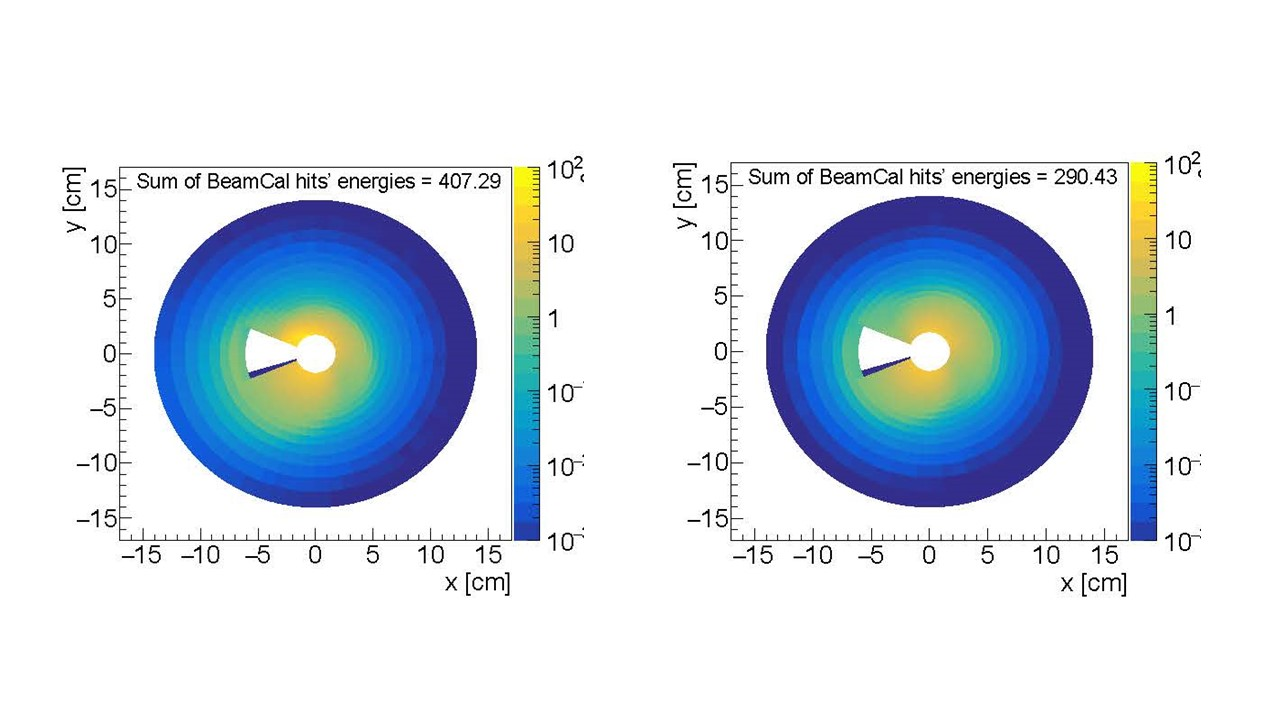
\includegraphics[width=1.0\hsize]{Integration/fig/BG_beamcal.jpg}
\caption{\label{fig:integration:beamcal}Beamstrahlung energy deposition in the BeamCal without (left) and with (right) anti-DID field for the large ILD version at ILC250. }
\end{figure}

\begin{table}\hspace*{-0cm}\small
\begin{tabular}{ l c c c }
\toprule
LAYER: & hits/BX & hits/BX & hits/BX/$cm^2$ \\
& No anti-DID & anti-DID & anti-DID \\
& mean $\pm$ RMS & mean $\pm$ RMS & mean $\pm$ RMS \\
\midrule
VXD 1: & 1400 $\pm$ 780 & 910 $\pm$ 360 & 6.6 $\pm$ 2.6 \\
VXD 2: & 970 $\pm$ 560  & 540 $\pm$ 210 & 4.0 $\pm$ 1.5 \\
VXD 3: & 150 $\pm$ 80   & 130 $\pm$ 60  & 0.21 $\pm$ 0.10 \\
VXD 4: & 110 $\pm$ 60   & 110 $\pm$ 50  & 0.18 $\pm$ 0.09 \\
VXD 5: & 44 $\pm$ 30    & 40 $\pm$ 26   & 0.04 $\pm$ 0.03 \\
VXD 6: & 39 $\pm$ 27    & 34 $\pm$ 24   & 0.04 $\pm$ 0.03 \\
\midrule
FTD 1: & 42 $\pm$ 30 & 38 $\pm$ 26 & 0.043 $\pm$ 0.030 \\
FTD 2: & 27 $\pm$ 19 & 24 $\pm$ 15 & 0.029 $\pm$ 0.019 \\
FTD 3: & 62 $\pm$ 45 & 40 $\pm$ 27 & 0.014 $\pm$ 0.010 \\
FTD 4: & 42 $\pm$ 33 & 25 $\pm$ 17 & 0.009 $\pm$ 0.007 \\
FTD 5: & 29 $\pm$ 23 & 18 $\pm$ 13 & 0.007 $\pm$ 0.005 \\
FTD 6: & 16 $\pm$ 13 & 9 $\pm$ 7   & 0.004 $\pm$ 0.003 \\
FTD 7: & 10 $\pm$ 8  & 6 $\pm$ 5   & 0.003 $\pm$ 0.003 \\
\midrule
SIT 1: & 51 $\pm$ 37 & 24 $\pm$ 16 & 0.0032 $\pm$ 0.0023 \\
SIT 2: & 49 $\pm$ 36 & 21 $\pm$ 12 & 0.0029 $\pm$ 0.0017 \\
SIT 3: & 77 $\pm$ 56 & 34 $\pm$ 24 & 0.0014 $\pm$ 0.0010 \\
SIT 4: & 71 $\pm$ 54 & 31 $\pm$ 21 & 0.0013 $\pm$ 0.0009 \\
\midrule
SET 1: & 39 $\pm$ 28 & 15 $\pm$ 10 & 0.00003 $\pm$ 0.00002 \\
SET 2: & 46 $\pm$ 36 & 18 $\pm$ 12 & 0.00003 $\pm$ 0.00002 \\
\bottomrule
\end{tabular}
\caption{\label{ild:tab:BGhits}Number of beamstrahlung hits per bunch crossing in the silicon trackers without (left) and with (middle and right) anti-DID field for the large ILD version at ILC250.}
\end{table}



A similar improvement is seen for the central detectors in table~\ref{ild:tab:BGhits}. The most affected are the inner layers of the vertex detector, where the background is equally shared between direct hits rather uniformly distributed, and back-scattered particles showing hot spots in azimuth. Background hits further away from the beampipe are dominated by direct $e^+e^-$ pairs. The anti-DID has little effect on direct $e^+e^-$ hits but helps to suppress back-scattered particles and associated hot spots in the central detectors.
%\textit{Comment also on TPC hits}.

For the small ILD version, the overall beamstrahlung background hit rates are reduced by $\approx$10\%  thanks to better confinement within the beampipe by the higher solenoid field of 4T.

%\textit{Add info on beamstrahlung effects on beamcal reconstruction and on HCAL occupancy near beampipe}

%\begin{figure}[t!]
%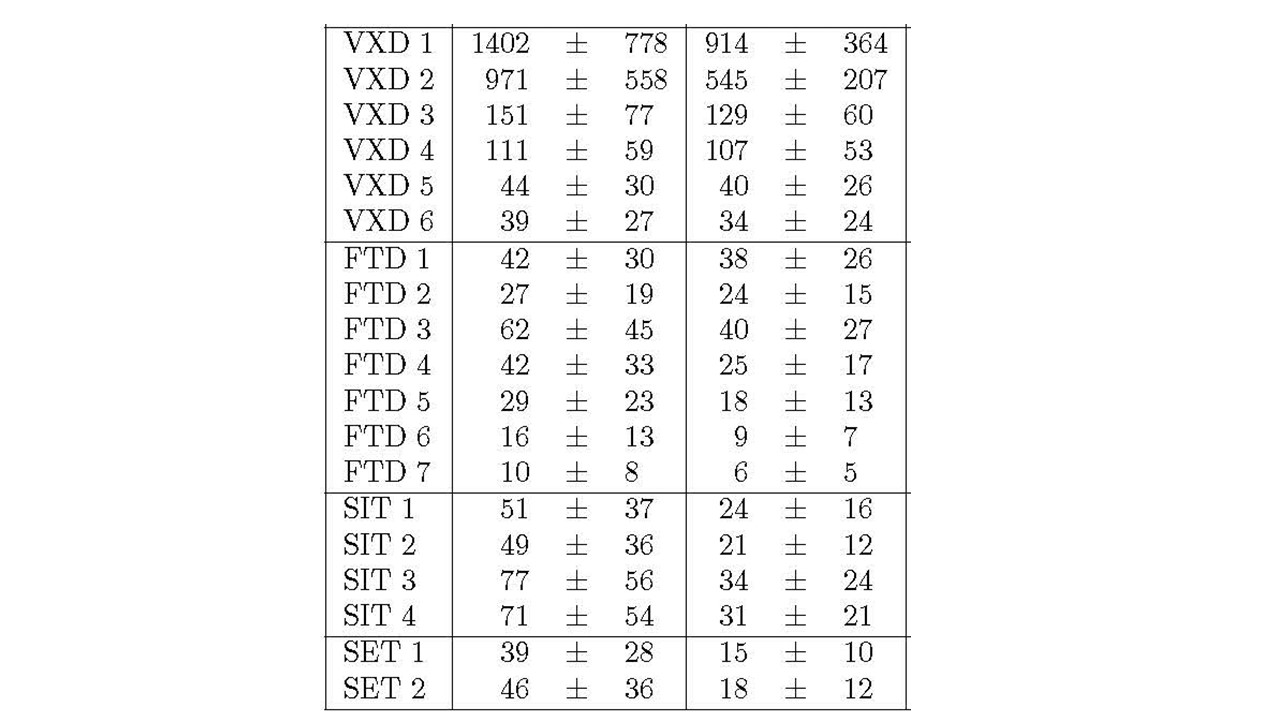
\includegraphics[width=0.8\hsize]{Integration/fig/BG_rates.jpg}
%\caption{\label{fig:integration:rates}Number of beamstrahlung hits per bunch crossing in the silicon trackers without (left) and with (right) anti-DID field for the large ILD version at ILC250. \textit{Give rates per $cm^2$ and transform figure into latex table.}}
%\end{figure}

\subsection{Halo muons}

The electrons and positrons of the beam halo produce high-energy penetrating muons parallel to the beam by interacting with beamline components such as collimators. Beam simulations~\cite{Keller:2019aak} predict that a fraction of $10^{-3}$ of the incident beam electrons hit a machine component of the beam delivery system and may therefore produce muons. Five magnetized muon spoilers and one optional larger magnetized muon wall are foreseen to deviate these muons outside the ILC experimental hall. The resulting rate of muons in ILD has been simulated for ILC250 and ILC500. 

\begin{figure}[t!]
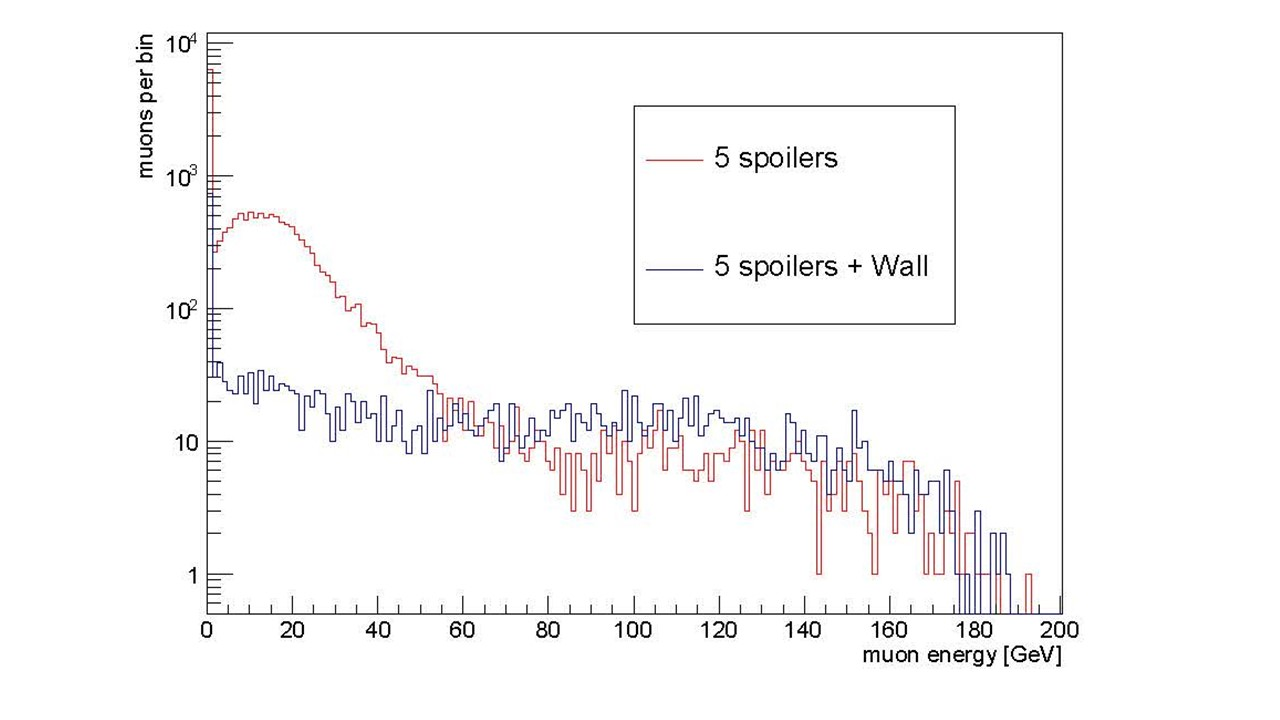
\includegraphics[width=1.0\hsize]{Integration/fig/BG_muons.jpg}
\caption{\label{fig:integration:muons}Energy spectrum of muons entering the ILC experimental hall for ILC500, normalized to a full single train of 2625 bunches assuming a beam halo fraction of $10^{-3}$. Red curve: muon filtering with 5 spoilers only; Blue curve: muon filtering with an additional muon wall~\cite{ild:bib:schuetz_thesis}.}
\end{figure}

Figure~\ref{fig:integration:muons} shows the energy spectra of the muons crossing the ILD detector for the two filtering options. The muon wall significantly reduces the flux of the lower energy muons below a few 10 GeV. At ILC500 the rate of halo muons crossing ILD is of the order of 4 (resp. 0.6) muons/BX without (resp. with) the optional muon wall. At ILC250 the corresponding numbers are of the order 1 and 0.03 muons/BX for the two filtering options, respectively.

These halo muons will affect the occupancy of the detector but should be easily identified and subtracted from the physics events using topological and timing information.

\subsection{Backscattered neutrons from beam dumps}

A potential additional source of beam-related background consists in particles back-scattered from the electron and positron beam dumps located 300m from the interaction point in both beam directions. This background is expected to be dominated by low energy neutrons which can propagate over a long distance. Their contribution has been fully simulated with FLUKA in the context of SiD, including a detailed description of the beamline up to the beam dump as well as of the dump system itself~\cite{ild:bib:schuetz_thesis}. The incoming neutron fluxes close to SiD are expected to be the same as for ILD and were interfaced to the ILD detector simulation to estimate their impact in the detector. The simulation was normalized to the dump of one full electron bunch on the +z side of the detector.

The total number of neutrons reaching the ILD detector region is found to be O($10^6$) per electron bunch dump. These neutrons have very low momenta of a few 10 MeV and most of them do not deposit a detectable signal in the detector. Their propagation in ILD was simulated and the map of their stopping points in the detector is shown in Figure~\ref{fig:integration:neutrons}. The results are in line of what is found for SiD~\cite{ild:bib:schuetz_thesis}: most neutrons are absorbed in the external layers of the ILD iron yoke, with a very small fraction reaching the external layers of the very forward calorimeters. Their energy depositions concentrate close to their stopping points: they are very small ($\approx$0.1 MIP in average) and asynchronous with respect to the bunch crossings. No visible signal is seen in the ILD vertex detector and central tracker. This indicates that the neutron background should not be a critical issue within its current state of understanding.

\begin{figure}[t!]
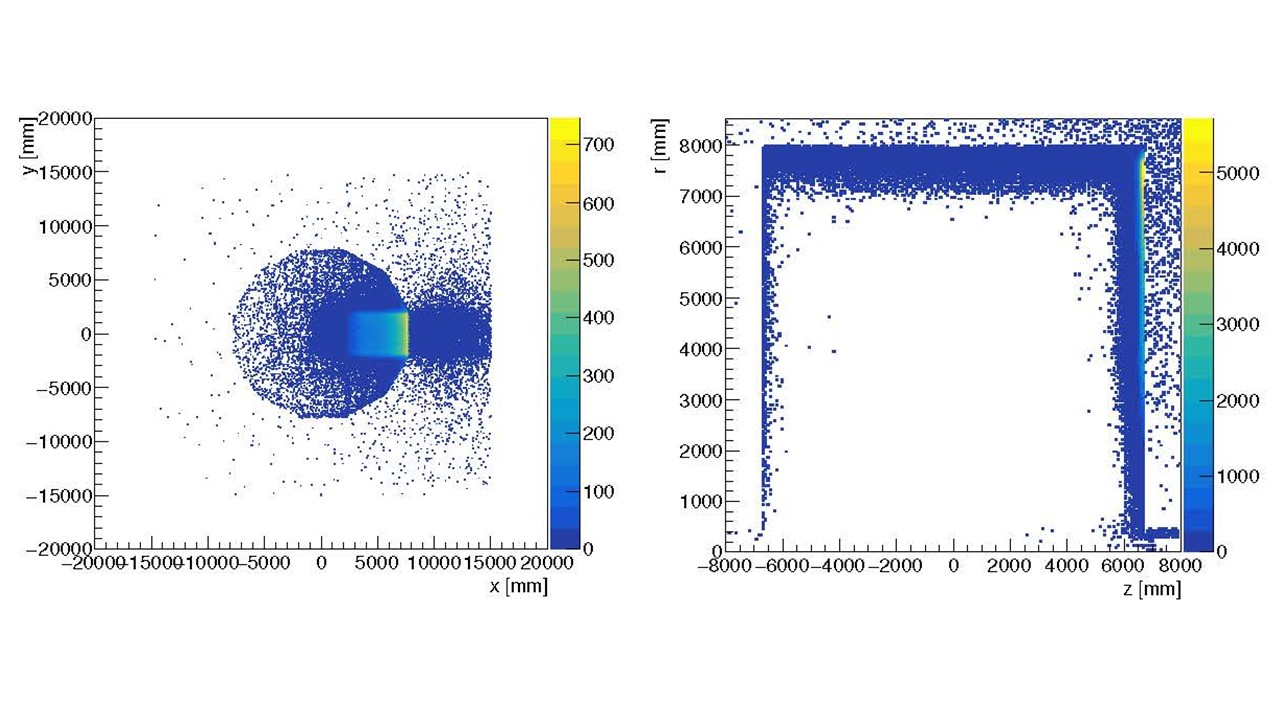
\includegraphics[width=1.0\hsize]{Integration/fig/BG_neutrons.jpg}
\caption{\label{fig:integration:neutrons}Map of the stopping points in ILD of neutrons back-scattered from the beamdump: transverse coordinates (left) and longitudinal coordinates (right). The map is normalized to the dump of one electron bunch on the +z side of ILD~\cite{ild:bib:schuetz_thesis}.}
\end{figure}

\vspace{2cm}
